\documentclass[11pt,a4paper]{article}
\setcounter{secnumdepth}{6}

\usepackage{standalone}
\usepackage{graphicx}
\usepackage[font=footnotesize]{caption}
\usepackage[noadjust]{cite}
\usepackage[toc,page]{appendix}
\usepackage{hyperref}
\usepackage{fullpage}
\usepackage{amsmath}
\usepackage{sidecap}
\usepackage{caption}
\usepackage{subcaption}
\usepackage[colorinlistoftodos]{todonotes}
\usepackage{csquotes}
\usepackage{parskip} % Spaces between paragraphs

\usepackage{pgffor} % foreach loops!

\usepackage[acronym]{glossaries}
\usepackage{geometry} % Used to adjust the document margins

% add binding margins
\geometry{bindingoffset=1cm}

\usepackage{xr}
\externaldocument[GR:]{../../report}



\makeglossaries
\renewcommand*\abstractname{Summary}

% http://www.tex.ac.uk/cgi-bin/texfaq2html?label=altabcr
\setcounter{MaxMatrixCols}{50}

% package name:
\newcommand{\means}{\texttt{MEANS}}
\newcommand{\pft}{\textit{p53}}
\newcommand{\py}{\texttt{python}}
\newcommand{\sympy}{\texttt{sympy}}
\newcommand{\plt}{\texttt{matplotlib}}
\newcommand{\mat}{\texttt{MATLAB}}
\newcommand{\eg}{\emph{e.g.}}
\newcommand{\ie}{\emph{i.e.}}

\newcommand{\sauliustodo}[2][]{\todo[color=cyan, #1]{\textbf{SL:} #2}}
\newcommand{\sisitodo}[2][]{\todo[color=yellow, #1]{\textbf{SF:} #2}}
\newcommand{\quentintodo}[2][]{\todo[color=red, #1]{\textbf{QG:} #2}}
\newcommand{\citationneeded}[2][]{\todo[color=brown, fancyline, #1]{\textbf{Citation Needed:} #2}}
\newcommand{\contrib}{\emph}
\begin{document}

\listoftodos
\newpage

\title{MEANS: a new python package for Moment Expansion Approximation, Inference and Simulation.\\
}
\author{Individual Report: Quentin Geissmann\\
\\    
\\
\\
\\
Supervised by Ann Babtie, Paul Kirk, Eszter Lakatos and Michael Stumpf\\
\\
\\
Theoretical Systems Biology Group,\\
Imperial College London
}
\date{\today}

\clearpage\maketitle
\thispagestyle{empty}
\newpage{}

\pagenumbering{roman}

% \begin{abstract}
% todo
% \end{abstract}

\tableofcontents

% our acronyms
\newacronym{ode}{ODE}{Ordinary Differential Equation}
\newacronym{mea}{MEA}{Moment Expansion Approximation}
\newacronym{lna}{LNA}{Linear Noise Approximation}
\newacronym{ssa}{SSA}{Gillespie Stochastic Simulation Algorithm}
\newacronym{cme}{CME}{Chemical Master Equation}
\newacronym{abc}{ABC}{Approximate Bayesian Computation}
\newacronym{sbml}{SBML}{Systems Biology Markup Language}
\newacronym{pypi}{PyPI}{the Python Package Index}

\newglossaryentry{maxord}
{
  name=max order,
  description={Maximal moment order. Max order always (regardless to the closure method) refers to the highest order of
  moments present in an ODE system resulting from Moment Expansion Approximation. In other words, moment expansion is closed at Max order $\mathbf{+1}$
   },
  sort=max order
}

\newpage{}
\printglossaries
\newpage{}
\pagenumbering{arabic}

\section{Introduction}

For our group project, we wrote a \py{} package for Moment Expansion Approximation, Inference and Simulation (\means).
Our group report explains our motivations, results and findings in detail.
Briefly, we provided a tool to model dynamic systems based on \acrlong{mea}\cite{ale_general_2013}.
Our implementation is very well documented, maintainable, extensible and user friendly.
It also performs considerably faster than previous implementations.

In the report herein, I describe some of my major contributions to the project.
First of all, I explain \emph{why} and \emph{how} the implementation of \acrlong{mea} was completely rewritten.
Then, I describe how parametric moment closure was translated from \mat{} prototype to be included in a unified framework in \means.
As explained in the group report, a considerable part of my work was also to improve the performance of \gls{mea}.
Here, I provide more details about the how this was realised.  
Finally, I explain the rationale behind integrating \acrlong{ssa} simulations in the package.

\section{Restructuring \acrlong{mea} Implementation}
As we attempted to read the \py{} implementation of \acrshort{mea} written by last year students\cite{babtie_moment_2013},
we were deterred by several points.
First of all, the code was often unnecessarily intricate and hard to understand.
Then, it was not organised in a very modular fashion.
Finally, established \py{} coding and documentation conventions\cite{_pep_????} were not respected.
These issues were limiting in so far as they reduced readability and made it hard to comprehend and improve the code.
We believe it would not have been possible, for us, to implement new features, such as parametric moment closure,
without having largely restructured the code in a first place.

My main individual contribution was to reforge the core implementation of \acrshort{mea} (as opposed to working on simulation and inference).
In the original code, symbolic computation relied on \sympy{}\cite{sympy_development_team_sympy:_2014}.
This library was efficient and well documented, thus we decided to also rely on \sympy{} for symbolic computations.
 
\subsection{Simplifying the Code}
We started by generating results from the original implementation and wrote ``regression tests''.
In this way, every time the code was amended, tests were run to ensure validity of mathematical results.

A major issue with the code was readability; in many cases, it was necessary to run the code in order to understand its role.
In this section, I illustrate, by three representative examples, how the original code was rewritten.

In the original code, the first step of the implementation of \acrshort{mea} was to generate a list of vectors of integers describing moments orders.
This list contained $c$ vectors for possible combinations of $d$ integers such as:\\
\[\mathbf{c} =(n_1, \dots, n_d) \forall{n_1, \dots, n_d \in \mathbf{N}}\]
satisfying the condition:\\
\[\sum_{j=1}^{d} {c_i}^j < o\]
up to moments of order $o$.\\

This was achieved through a very intricate recursive function which was extremely difficult to read and modify.
Instead, we used the \texttt{product()} function, in the standard module \texttt{itertools},
to generate all $o^d$ combinations of $c$ vectors of length  $d$, in one single line of code.
It was then trivial to filter the resulting list in order to keep only vectors with a sum lower or equal to the highest order of moments $o$.

Another striking example of complexity of the original code what the calculation of partial derivatives.
In order to compute the result of eq.~7 of \gls{mea}\cite{ale_general_2013} it is necessary to calculate\\
\[\frac{\partial{}^\mathbf{n} a_l(x)}{\partial{}\mathbf{x^n}}\]
where,\\
\[\partial{}^\mathbf{n} = \partial{}^\mathbf{n_1+\dots{}+n_d}\]
\[\partial{} \mathbf{x^n} = \partial{} x^n_1 \dots{} \partial x^n_d\]

In the original code, the property:
\begin{equation}
\label{eq:partial}
\frac{\partial{} ^ 2 f(x,y)}{\partial x \partial y} =
\frac{\partial{} \frac{\partial{} f(x,y)}{\partial x}}{\partial y} =
\frac{\partial{} \frac{\partial{} f(x,y)}{\partial{} y}}{\partial{} x}
\end{equation}
was used to pre-compute partial derivatives starting from low order and using the result to derive higher order.
All derivative were stored in a three dimensional hierarchical construct (named \texttt{`damat'}).
Further in the code, it was necessary to perform  tedious index calculations to
retrieve partial derivatives for each moment order combination.
This was both hard to understand the structure of \texttt{damat} and to retrieve values from it.
In addition, this type of unusual structure was deprecated in the next version of \sympy{}.
Investigating the documentation of \sympy, it appeared that it was in fact possible to directly compute partial derivatives
with respect to arbitrary number and order of variables.
For instance, \texttt{sympy.diff(y,x1,x1,x2)} would return $\frac{\partial^3 y}{\partial x_1^2 \partial x_2}$.
This was later optimised (see section~\ref{sec:optimisation}).

A last example is the use of symbols describing moments (raw and central) in the original code.
Everywhere a symbol describing a moment was needed, it was necessary to create a string from a vector of orders with the correct naming convention.
For example, a raw mixed moment could be described by a string such as \verb"x_123".
``Hard-coding'' the names and naming conventions rendered it very difficult and error-prone to change the notations for symbols.
For instance, judged better to use \verb"x_a_b" instead of \verb"x_ab" as symbol for a raw moment of order ($a$ and $b$)
because the latter notation would be ambiguous if ever moments were computed for orders higher than ten (\eg{} \verb"x_111" could mean either \verb"x_11_1"  or \verb"x_1_11").
Instead, in \means, two lists of `Moments' objects are created instead of two list of vectors of orders (one for raw moments and one for central moments).
Each `Moment` contains a variable for `symbol` and a vector of orders.
Firstly, this implies that symbol are when creating a Moment object.
Secondly, future developers do not need to be aware of the naming convention.
Lastly, this approach renders later substitution of symbols by integers or other symbols unnecessary.
In contrast, in the original code, central moments were encoded as \verb"ym_ab" and then
converted to \verb"yxN" (where \verb"N"  is a positive integer),
and $0^{th}$ order raw moments had to be converted to $1$.
Our approach allows to allocate the final symbol (or value) once for all at the start, which greatly simplifies the code.

\subsection{Using Modularity}

The original implementation had very little modularity.
There were a few functions, which were essentially executed once.
However, there were many repeated processes in the code.
For instance, two Taylor expansions used the same principles,
so it was often possible to write functions that several parts of the code could use.
This obviously shortened and organised the code, but also made it much simpler to profile and improve the it.
 
In addition, no classes were used.
Object oriented programming is a powerful concept allowing to organise and reuse code very efficiently.
In the original code, there were a large function to perform \gls{lna}, and another one to perform \gls{mea}.
However, some of the tasks performed by both methods rely on the same principle: using a model as an input and generating a set of \glspl{ode} as an output.
Therefore, it was very advantageous to make a base class for all approximation method, from which both \gls{lna} and \gls{mea} derived.
In addition, object oriented programming allowed us to define custom data structures with their own methods.
For instance custom \texttt{ODEProblems} and \texttt{Moments} objects were very helpful to represent mathematical concepts.

\subsection{Using \py{} Standards}
The original code uses indexed for loops (like in \texttt{C}).
However, in \py, ``foreach'' loops are  standard and are much more efficient and readable.
In addition, advanced syntactic feature of \py{} such as ``list comprehensions''  and mapping,
which are very concise and efficient, where not used.
For instance, in the original code, filtering a vector for values higher then six was done like:

\begin{verbatim}
vector = [1, 5, 7, 8, 3]

filtered_vector = []
for i in range(0, len(vector)):
    if vector[i] > 6:
        filtered_vector.append(vector[i])
\end{verbatim}

In \py{} standards, the can be in one line:

\begin{verbatim}
filtered_vector = [v for v in vector if v > 6]
\end{verbatim}

This may look insignificant for a simplistic example, but it becomes very hard to manage nested loops (which were numerous) with the former version.
Moreover, it is more efficient to use iterators rather than indexing.

In \means, we took advantage of these features to improve the code.
In addition, the entire code was documented following established standards.
This allows, for instance, to automatically generate online documentation for developers and users.


%\cite{ale_general_2013}

\begin{table}[tbh]
\caption{\emph{Examples of variable name choices.}
Comparison of some  variable names between original \py{} code, our package(\means) and the reference publication.
}

\begin{center}   
    \begin{tabular}{ | l | l | r|}
    \hline
    \bf{Publication\cite{ale_general_2013}} & \bf{Original} & \bf{\means}\\
    \hline
    \hline
    $\frac{d_{\mu}}{dt}$ & \verb"M" & \verb"dmu_over_dt"\\
    \hline
    $\mathbf{n\choose{k}}$ & \verb"f2" & \verb"n_choose_k"\\
    \hline
    $ (-1)^\mathbf{{n-k}}$ & \verb"f3" & \verb"minus_one_pow_n_minus_k"\\
    \hline
    $\mathbf{n_1    , n_2, ..., n_d}$ & \verb"counter" & \verb"n_counter"\\
    \hline
    $\mathbf{k_1, k_2, ..., k_d}$ & \verb"mcounter" & \verb"k_counter"\\
    \hline
    \end{tabular}
\end{center}
\label{tab:varnames}
\end{table}

Another important, but often neglected, aspect of readability is the choice of variable names.
Having explicit self explanatory variable names often reduces cognitive load.
Modern code editor allow completion of variable name, so it is not limiting to use long names.
We aimed to name variables according to the symbols in the original publication\cite{ale_general_2013}.
Table~\ref{tab:varnames} represents a few examples of how we chose variable names.


\section{Parametric Moment Closure Implementation}
Implementation of moment closures using parametric distributions was done in collaboration
with Sisi Fan because prototypes were available in \mat{}\cite{lakatos_preparation_2014}. She had experience using \mat{},
whilst I had more practice with \py{}.
Here, I only describe my decisions about the implementations in \py{}.

All closure methods essentially replace higher order (\gls{maxord}~+~1) raw moment symbols with expressions000 depending on lower order moments (or constants).
For parametric closure, raw moments are expressed in terms of lower order moments.
In addition, for univariate distributions, mixed raw moments are always set to $0$.
In the \mat{} prototype, all closures were implemented independently without using a explicit common structure.
In addition, the default (scalar) closure was implicit and had a singular behaviour.

In \means, we have unified all closure methods in a common base class (\texttt{ClosureBase}).
The base class implements all methods that all closures will use (\ie{} substitutions, setting cross terms to $0$).
Then, only the method to compute raw moments has to be specialised in subclasses.
This general framework facilitated optimisation and will greatly simplify the task of researchers willing
to implement closure methods for new distributions.

\section{Optimisation of Symbolic Computations}

\label{sec:optimisation}

In this section, I detail how optimisations of symbolic calculation were performed (fig. ~\citationneeded{find me} in the group report).
As a reminder, the number of equations generated by \gls{mea} for a system with $s$ species and up to \gls{maxord} of $o$
is defined by:
\begin{equation}
    \text{Number of equations} = {{s + o} \choose {s}} - 1
    \label{eq:number_of_equations}
\end{equation}

As a consequence, the symbolic computations become extremely costly if the number of species or \gls{maxord} increase.
Therefore, it was extremely important to optimise performance of \gls{mea} in order to make it available for models with more species.

\subsection{Profiling}
Optimisation was realised using \py{} profiling tools.
This provides valuable information such as how many times a function is called, and how long, in total,
the interpreter spent ``in'' this function (which is yet another reason use modularity and write functions).
Figure~\ref{fig:profile} represents the result of such a profile obtained during development.


\begin{figure}[tbh]
\begin{center}
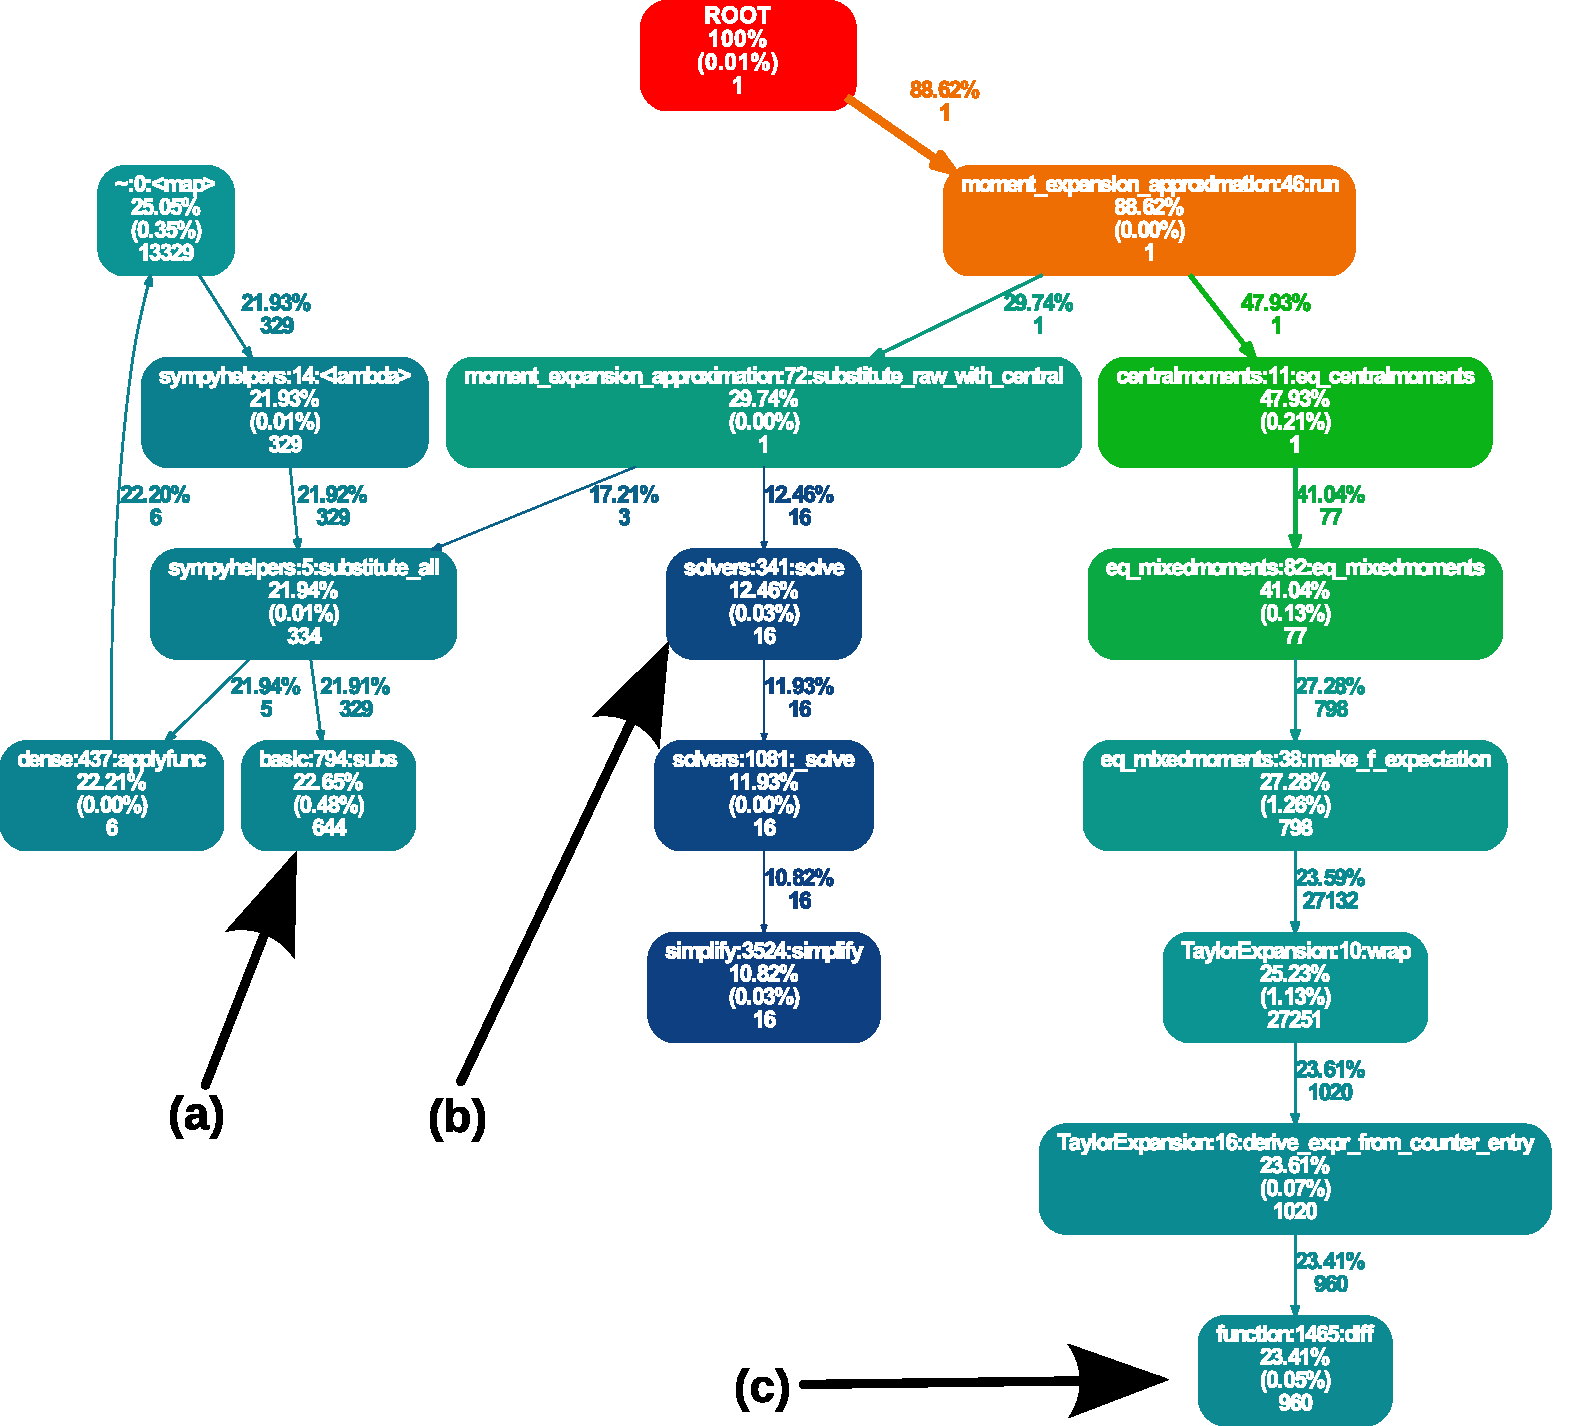
\includegraphics[width=0.83\textwidth{}]{profile.pdf}
\caption{\emph{Simplified profile of \gls{mea} using means.}
Each box indicates a function.
Colour arrows indicate a ``caller $ \rightarrow $ callee'' relation.
The first row in each box is the name of the function (prefixed with the module name and the line number).
The second row indicates the total time spend calling this function (directly or indirectly).
The last row is the total number of time a function has been called.
Black arrows indicate \sympy{} functions with large footprints which are explicitly called by our package.
This example profile suggests that symbol substitution could be an issues (a).
The function \texttt{sympy.solve()} also seems to have a large footprint (b).
Finally differentiation (\texttt{diff}) is coslty (c).
Altogether, the interpreter spent approximatively $60\%$
of the runtime in these three functions.
Note that this specific profile has been pruned to facilitate representation.
}
\end{center}
\label{fig:profile}
\end{figure}

 
\subsection{Improving Performance Iteratively}
In this section, I detail the nature of the optimisations performed in section\citationneeded{} of the group report.
The relevant figure is reproduced as figure ~\ref{fig:mea_speed} of the document herein.

\begin{figure}[tbh]
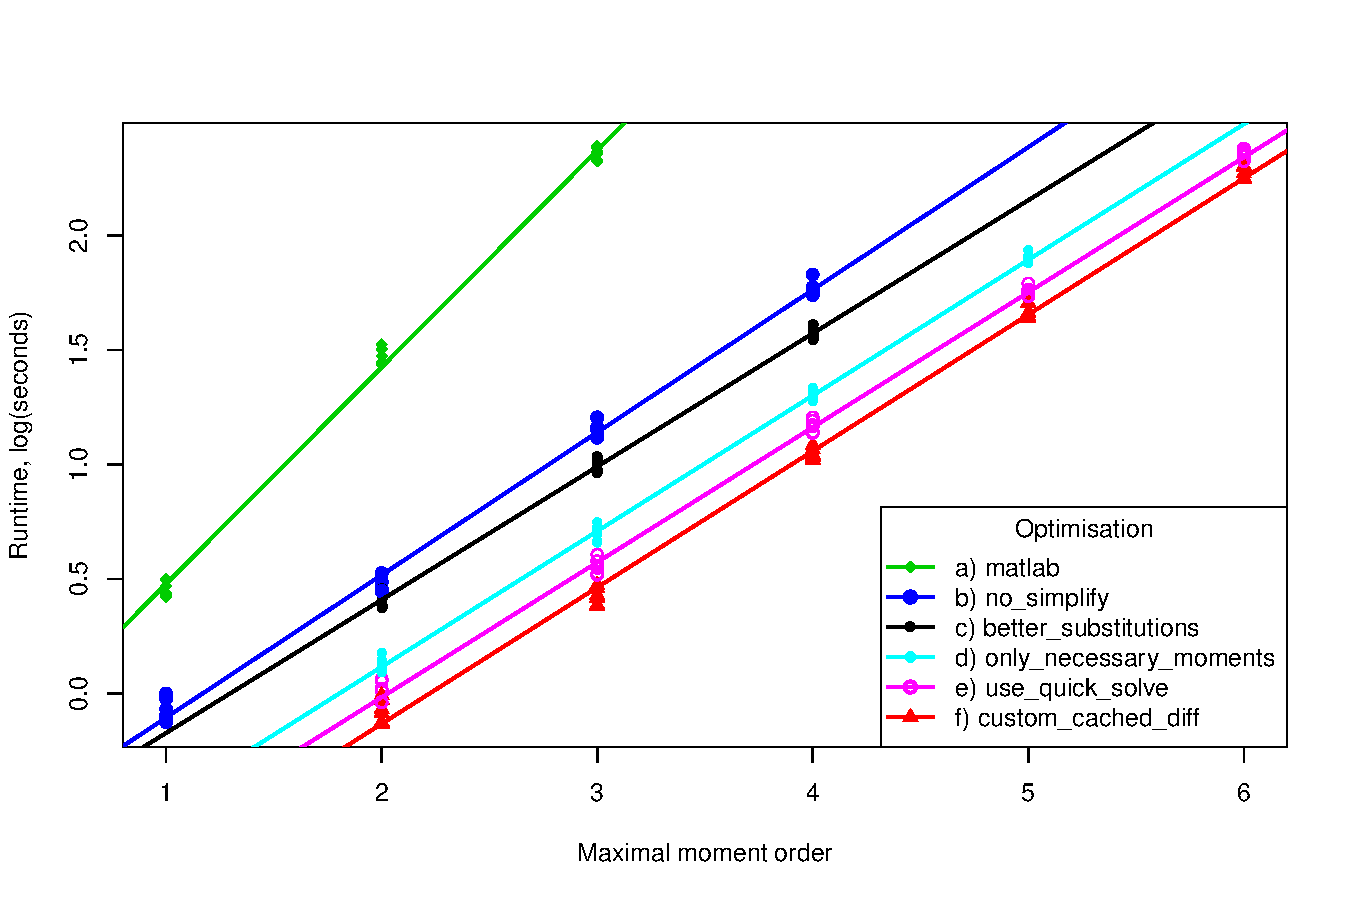
\includegraphics[width=0.95\textwidth{}]{mea_speed.pdf}
\caption{\emph{Cumulative performance improvement of symbolic
calculations resulting from optimisation}.
The processing time for computing log-normal closure on \pft{} model with different \gls{maxord}s were measured for original Matlab implementation (a) and different optimisations (b$-$f).
In a first place, the calls to \texttt{sympy.simplify()} were removed (b).
Then, \texttt{sympy.xreplace()} was used instead of \texttt{sympy.substitute()} (c).
Computing a rectangular matrix containing expressions for all moment was more efficient than generating a square matrix to later remove unneeded expressions (d).
Implementing a simplified equation solver instead of using \texttt{sympy.solve()} also resulted in a significant speed-up (e).
Finally, caching (memorisation) \texttt{sympy.diff()} allowed even better performance.
The time complexity appears exponential ($O(2^k)$, where $k$ is the maximal moments order) in every case,
Nine replicates were performed on the same CPU.
For optimisation c$-$f, values corresponding to \gls{maxord} moments lower than two were removed because of
the inherent inaccuracy in measuring very short durations.}
\label{fig:mea_speed}
\end{figure}


The first optimisation step involved removing the ``expression simplification'' heuristic.
In the original code (from both publication\cite{ale_general_2013} and last year's MSc project\cite{babtie_moment_2013}),
the right-hand-side equations were simplified in order to produce shorter text file results.
However, this was slow and did not benefit subsequent simulations and inference.
For large expressions, simplification also had an large memory footprint and was likely to fail.
This removing simplification routines significantly improved the scalability of the method (see fig.~\ref{fig:mea_speed}b).

The next bottleneck was the choice of substitution functions.
As a part of \gls{mea}, it is necessary to replace raw moment symbols by expressions depending on central moments.
Performing substitution can be done using the \texttt{substitute()} function from \sympy, but this is designed to substitute expressions by other expressions.
In most cases, we only had to substitute atomic symbols by expression.
For this purpose, the \texttt{xreplace()} function was a much more appropriate alternative which resulted in a better scalability (see fig.~\ref{fig:mea_speed}c).

In the original implementation, a matrix of central moment expression of size
\[(n-s) \times (n-s + 1)\]
where,
$n$ is the number of equations (see eq.~\ref{eq:number_of_equations}) and
$s$ is the number of species,
was directly generated for scalarclosure.
However, when for parametric closure, a matrix of size $(n_2-s) \times (n_2-s + 1)$,
where,
\[n_2={{s+o \mathbf{+1}} \choose {s}} -1\]
was generated.
The $n_2 - n$ rows corresponding to higher-order moments were unused and eventually deleted.
In contrast, our implementation generates a $(n-s) \times (n_2-s + 1)$ matrix regardless of the closure method.
In addition to making the code more readable, consistent and flexible, this improved overall performance (fig.~\ref{fig:mea_speed}d)
for cases where closure is applied whilst keeping the default closure computation fast.

Another simple way to improve computation time was to remove calls to the function \texttt{solve()} which was only used in straightforward cases
(\eg{} solving: $x + 2y = z$ for $x$).
It was therefore much more efficient (fig.~\ref{fig:mea_speed}e) to use trivial arithmetic to find solution.

Finally, partial derivation of expression over several variables and order is extensively performed during the approximation.
Generally, these type of differentiations can be simplified several differentiation of first order (see eq.~\ref{eq:partial})
One advantage, is that, when needing to calculate two derivatives such as: $\frac{\partial{} ^ 2 f(x,y)}{\partial{} x \partial{} y}$ and $\frac{\partial{} ^ 2 f(x,y)}{\partial{} x^2}$,
one can precompute $\frac{\partial{} f(x,y)}{\partial{} x}$ and use it for both calculation.
In our implementation, we have use a procedure known as \emph{memoization} that, briefly, permits to store the results of a function call in an associative array.
Then, the next time this function is called with the same arguments, it will return the stored results instead of recomputing it.
This also resulted in an overall performance improvement (fig.~\ref{fig:mea_speed}f).

Interestingly, the slopes between, optimisations a ($0.95$) and c ($0.58$), and b ($0.62$) and c were significantly different ($p-value <10^{-15}$ and $p-value = 3 \times 10^{-4}$, respectively;
t-test on the slopes of the linear regression). This indicates that optimisation c ``scales'' better that b and a.
No significant difference was found between the slopes of the subsequent optimisations (c$-$f).
However, the intercepts were significantly smaller between each consecutive optimisations after c) ($p-value < 10^{-6}$ for all; t-test on the intercepts of the linear regression).

Compared to the original \mat{} implementation, these improvement are very significant. We estimate than, for computing \gls{mea} with log-normal closure up to \gls{maxord}
of 8 in the \pft{} system, our implementation is approximately 5000 faster.

\section{Implementation of \acrlong{ssa}}
Finally, when we started to evaluate the accuracy of \gls{mea}, we realised that it was necessary to compare simulation results to \gls{ssa} average\cite{gillespie_general_19706}.
Considering the number of parameter sets we needed, it was not practical to generate average trajectories using an external programs.
We therefore implemented our own version of the exact, direct algorithm.
The algorithm is quite simple, so it was quick to provide a basic implementation.
The most important for our research was to integrate stochastic simulations consistently with the rest of the package.
For instance, it needed to return the same type of objects as simulation based on approximation.
In addition, it was necessary that \gls{ssa} simulations could return empirical moments on collections trajectories, which allows to compare mean, variance, covariance, and so on, between simulations.
If, in the future, a faster implementation of \gls{ssa} is needed, it should be straightforward to optimise this code.

%%%%%%%%%%%%%%%%%%%%%%%%%%%%%%%%%%%%%%%%%%
A CONCLUDING REMARK PLEASE (I ENJOYED THE PROJECT, TNAK YOU THE MASTERSSSSSS :p)

\newpage{}
\bibliography{report.bib}{}
\bibliographystyle{ieeetr}

\end{document}